% This is samplepaper.tex, a sample chapter demonstrating the
% LLNCS macro package for Springer Computer Science proceedings;
% Version 2.20 of 2017/10/04
%
\documentclass[runningheads]{llncs}
%
\usepackage{graphicx}
\usepackage{xcolor}
\usepackage{wrapfig} % Added by Sid to wrap figure around text
\usepackage{hyperref} % added by Sid for hyperlinks 

% Used for displaying a sample figure. If possible, figure files should
% be included in EPS format.
%
% If you use the hyperref package, please uncomment the following line
% to display URLs in blue roman font according to Springer's eBook style:
% \renewcommand\UrlFont{\color{blue}\rmfamily}

\begin{document}
%
\title{Toward A High-Performance Emulation Platform for Brian-Inspired Intelligent Systems \\ Exploring Dataflow-Based Execution Model and Beyond}
%
%\titlerunning{Abbreviated paper title}
% If the paper title is too long for the running head, you can set
% an abbreviated paper title here
%
%\author{Sihan Zeng\inst{1} \and
%Jośe Monsalve \inst{2} \and
%Siddhisanket Raskar\inst{2}}
%
\author{Sihan Zeng 
\and Siddhisanket Raskar
\and Jose Monsśalve }

\institute{Carnegie Mellon University \and Univeristy of Delaware}

%\authorrunning{Zeng et al.}
% First names are abbreviated in the running head.
% If there are more than two authors, 'et al.' is used.
%
%\institute{Carnegie Mellon University \and
%Univeristy of Delaware \\
%\email{sihanzen@andrew.cmu.edu\inst{1} \and josem@udel.edu\inst{2} %\and sraskar@udel.edu\inst{2}}}
%

\maketitle              % typeset the header of the contribution
%
\begin{abstract}
Brain inspired computing is a novel computing technology based on neural morphological engineering, which draw lessons from methods of human brain information processing and storage. Combining with the high-performance computing (HPC) platform, they constitute the foundation of general artificial intelligence. However, current brain HPC platforms generally suffer from slow speed, poor scalability and high energy consumption, which severely restrain the potential of brain inspired computing and circumscribe the development of general artificial intelligence. To solve these problems, dataflow model was first proposed in 1970s, providing a novel idea for the development of HPC. In addition, the dataflow model shares similar information processing mechanism with human neural system, which makes the dataflow model naturally suit the emulation of brain-inspired computing. Based on the contemporary progress of dataflow model, the Codelet model was proposed. Through the fine-grained asynchronous program execution and resource allocation, the Codelet model successfully realized the distributed computing on the heterogeneous system, effectively improved the computing power and speed, and open up a new path to overcome the shortcomings of the existing high-performance computing technology.
Therefore, based on the Codelet model, we propose a dataflow-based emulation platform, aiming at providing high performance computing technology support for general brain-inspired intelligent system, as well as using the characteristics of dataflow model to fully explore the potential of brain-inspired intelligence. As an example, we will select a convolutional neural network (LeNet5) that already has a spectacular user base to initially verify the superiority and feasibility of our proposal.


\keywords{First keyword  \and Second keyword \and Another keyword.}
\end{abstract}

\section{Introduction}
\label{sec:intro}
The human brain is one of the most complex processing systems known to us. Despite the progress that has been made in understanding its behavior and functionality, there are many aspects of it that are still unknown. One major breakthrough was the discovery of the neural network and, later on, the introduction of Artificial Intelligence in the late 50s which was heavily influenced by real neural networks. On the other hand, computer systems have been evolving in parallel with AI, and it has been possible to obtain major improvements on computations that the brain itself is not capable of. As an example, computers can perform billions of mathematical computations per second, beating up humans by a wide margin, but mainstream architectures of computer systems do not have the ability to achieve the capacity of the brain, specially in areas like patter recognition, learning capabilities and self adaptation. 

Brain-inspired computing is a novel information processing technology, which learns from the basic rules of how human brain processes information and makes improvement on the existing computing technology based on these rules. Brain-inspired computing covers a wide variety of topics such as software algorithms and hardware systems. In the case of software algorithms, the most pervasive application is the Artificial Neural Network (ANN). The ANN consist of neurons, connections and hierarchical architectures inspired by neuron systems found in human brains. Although early ANNs were relatively simple and had limited functionality researchers have deepened the neural networks by increasing the number of layers and the complexity of their connection, resulting in the concept of "deep learning" developing rapidly. This has enabled a major breakthrough on massive cognition tasks such as speech recognition and image recognition leading to great advances like self driving cars. However, as the neural networks becoming deeper, the number of neurons and connections drastically increases, which inevitably results in the more urgent needs of computing power. For example, the GoogLeNet, proposed by Google Brain, consists of 22 layers and more 5 million parameters. 

It is then fair to ask what has lead great advances in the areas of AI (and related) in the recent years, despite of a decades long history of these fields? The answer can be easily found when the history of parallel computer systems and brain-inspired computation are placed side by side. Parallel computing was introduced around the mid 60's and great advances were made in parallel computing in the 70's and 80's. Still, the success of sequential computation that was driven by an aggressive technology scaling, as well as a well defined model of computation, lead parallel computing through a dark period in the 90's that was well described by Ken Kennedy in his article "is parallel computing dead?" \cite{kenedy96}. At the same time, interest in AI decreased due to the lack of viability in terms of computation and emulation. However at the beginning of the 2000's single core architectures starting to experience major limitations in power consumption and memory bandwidth, resulting in a degraded scaling of systems. These brought up interest on parallel computing again, and in a second spring for parallel systems and unconventional computer architectures. At the same time the internet revolution and other aspects brought back interest in AI and brain inspired computation. It is now clear that being able to emulate the behavior of these huge neural network requires multiple CPUs, or even GPUs to perform the parallel computing. The wide availability of both, is driving the world to a second spring of AI and parallel computing that could have major implications at all levels of our society. 

However, it has been challenging to build a brain-inspired computing system using parallel computing. Among many more, there are three challenges that are critical: The first challenge lies in determining the granularity of the parallelism given the system architecture and size of the application. The second challenge is how we can build a brain-inspired computing system that scales up with the number of cores by using fine-grain parallel schemes. The third challenge is how to measure the effectiveness of such system and how to justify and locate the source of changes in effectiveness and performance of brain-inspired applications. 

For the first challenge, a decision should be made between coarse-grained and fine-grained parallelism. Today’s widely adopted parallel programming models, including MPI, OpenMP and other derived models, are all extended from the Bulk Synchronous Parallel (BSP) model. Nevertheless, BSP-like models have shown serious bottlenecks in part due to the cost of synchronization which scales up with the size of the system. This is worsen by the strict sequential memory models enforced by current computer architectures, and the variability in core's behavior and execution time, among other aspects. Resulting in poor scalability with the number of cores, leading to the increase in the CPU idle time, and reducing the desired performance gain expected in parallel systems. Additionally to these, and possibly the most negative drawback lies in that it model does not solve the bottleneck of memory access under the traditional Von Neumann architecture, which severely restrict the potential of brain-inspired computing systems and software. Therefore, it is necessary to move away from coarse grain parallelism in order to address the above bottlenecks. We believe that find-grained parallelism could increase the ability of parallel computers to deliver performance scaling, and providing high-performance parallel acceleration for brain-inspired computing.
Then comes the second challenge, how can we build a brain-inspired computing system based on fine-grained parallelism. Fortunately, the dataflow model of computation proposed in 1974 by Jack Dennis \cite{JackB74} provides a parallel execution architecture that supports fine-grained parallelism.

In the dataflow model of computation, the execution of instructions is not controlled by the program counter, but rather it depends on whether the required input data is available or not. This is, when all the input data of an instruction is available, the instruction is then ready to be executed. When the instruction has finished execution, the output becomes available to the following instructions that depend on such result. This asynchronous execution manner of the dataflow model is able to provide the fine-grained parallelism as low as instruction level. For this reason, dataflow models not only provide fine-grain synchronization, but also the data dependency pattern presented between instructions is similar to the signal transmission mechanism between neurons in the artificial neural networks. This empowers dataflow based execution model and architectures with the capability to emulate the existing artificial neural networks, as well as the potential to introduce more sophisticated interaction mechanisms between neurons.

The Codelet model, proposed by Guang R. Gao in 2011, is a fine-grained parallel Program Execution Model (PXM) that derives from the idea of asynchronous execution of the dataflow model, while borrowing ideas and concepts of the Von Neumann model. Compared to the dataflow model, the extension of Codelet model lies in: First, Codelets are not single instructions, but a collection of instructions that are functional and side effect free. These instructions form a task of the Codelet Graph, and could be executed in Von Neumann architectures. In addition Codelets are not only data-driven, but also event-driven. In Codelet model, the execution of a program depends not only on the availability of input data but also on the machine resources and events. Second, it uses threaded Procedures, which are containers for the execution environment of Codelets and that asynchronous function calls that use continuation signals to return values to codelets in the Caller's environment. Codelets still rely on fine-grained parallelism that enables more flexible resource allocation, but they use argument fetching data-flow, which assembles an architecture closer to Von Neumann architectures that are widely available and studied. Therefore, it is of great significance if we could study the codelet model when applied to brain-inspired computing.

Finally, for the third challenge, we need to apply our system to benchmarks that are classical representations of artificial neural networks to indicate the practical advantage of our system. Also, we need to provide evidence about how computation are accelerated during execution, in order to support the arguments about fine-grained parallelism. 

Aiming at addressing the above-mentioned challenges, this paper mainly have three contributions as follow:
\begin{itemize}
    \item We use the fine-grained multi-thread parallelism of Codelet model as an initial attempt to solve the technical bottleneck faced by the existing coarse-grained parallelism and provide higher performance parallel acceleration for the simulation of artificial neural network.
    \item To our knowledge, this is the first work that applies the Codelet model to brain-inspired computing, especially to the simulation of neural networks, providing a novel path for high-performance brain-inspired simulation platforms.
    \item We evaluate our system based on the most pervasively used neural network, LeNet5, to demonstrate the feasibility and superiority of the codelet model. We also conduct study on the source of effectiveness of fine-grained parallelism by profiling the execution of our system. 

\end{itemize}



\section{Related Work}
\label{sec:related}
Currently, the most commonly used neural network simulation framework is Tensorflow developed by the Google brain. Tensorflow executes neural networks in the form of dataflow graphs (DFG). The nodes in the DFG represent math operations, and the edges in the DFG represent the interactions between operations. Tensorflow can flexibly deploy the computation task of a neural network on arbitrary servers with CPUs and GPUs, or on mobile devices. Specifically, the DFG is partitioned into several parts and the computation of each part are allocated to different devices for execution.
Due to the growing model size of the neural networks, plenty of research focus on the parallel acceleration of training and inference of the neural networks. Yunji Chen discovered that the memory footprint of convolutional and deep neural networks (CNNs and DNNs), while large, is not beyond the capability of the on chip storage of a multi-chip system. They developed DaDianNao, a custom multi-chip machine-learning architecture that enables high-degree parallelism of the execution of neural networks at a reasonable area cost. Song Yao et al. started from the algorithm aspect of neural networks. They leveraged pruning to reduce the amount of connections, as well as quantification to reduce the memory usage of each parameter. At the same time, Yao adopted software and hardware co-optimization strategy, which can provide faster acceleration of the execution of neural networks from the hardware aspects. On these basis, Yao et al. proposed Efficient Speech Engine (ESE) and Efficient Inference Engine (EIE).
Generally, the optimization of parallel acceleration of neural networks can proceed from two aspects - structure and algorithm. The former achieves parallel computing with less overhead by changing computation mode and memory access mode. The latter increase the execution speed and storage efficiency of the neural networks by reducing the amount of connections and uneven quantification of parameters. In the future, with the rapid evolution of neural networks, various new structures and algorithms aimed at efficiently parallel acceleration are still evolving rapidly.
With respect to the works about dataflow model. Intel recently released an exascale dataflow engine, i.e. configurable spatial accelerator, which implements the dataflow program execution model on the hardware level. The engine is primarily consist of several computation processing elements, interconnected networks and in-fabric storage elements. This structure of CSA is physical implementation of the underlying abstract hardware of coldelet model, which enables CSA to support the similar task suit for codelet model such as neural networks execution.  



\section{The Codelet Model}
\label{sec:model}

\begin{wrapfigure}{l}{0.25\textwidth}
    \centering
    \caption{Figure 1}
    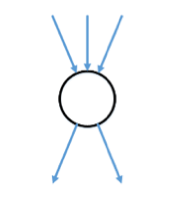
\includegraphics[width=0.25\textwidth]{Fig/figure1.png}
\end{wrapfigure}


%\vspace{1.5cm}


The Codelet model is a fine-grained multi-threaded parallel program execution model based on data flow architecture. Codelet is the finest granularity of parallel units. Each Codelet contains a set of machine instructions, as shown in Figure 1. During the scheduling process, each Codelet is considered as atomic operation. Once the CPU executes a Codelet, it will not be interrupted or migrated to another CPU by the scheduling policy until all the instructions contained in the Codelet are finished, i.e. non-preemptive run. Moreover, since CPU does not have to pay for the overhead of switching between Codelets (saving context, registers, etc.), the Codelet model achieves high efficiency while maintaining fine-grained threading.
%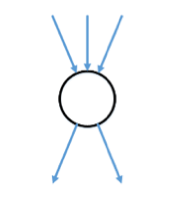
\includegraphics{Fig/figure1.png}

\subsection*{Firing Rules}
When a Codelet receives signals from each of the preceding Codelets (i.e. all dependencies are satisfied), the Codelet will be fired - sent to CPU for execution by scheduling policy. The execution of a Codelet consists of three steps: 1) resetting all predecessors, 2) executing internal machine instructions, 3) generating output results, releasing machine resources and sending signals to subsequent Codelets.
\subsection*{Codelet Graph (CDG)}
Since Codelets are data / event driven, Codelet models do not follow the order of a list of instructions, but instead rely on data / resource dependencies. After the completion of a Codelet, it will produce the corresponding output and release machine resources, while other Codelets may depend on such resources or data. The directional connected graph determined by these dependencies is Codelet Graph (CDG). The nodes in the CDG represent Codelets, the directed edges represent the data dependencies between Codelets, and Figure 2 shows a Codelet Graph.
\subsection*{Threaded Procedure (TP)}
To achieve a higher degree of concurrency, CDG can be partitioned into several subgraphs based on function or execution duration for parallel execution on different CPUs. The Threaded Procedure (TP) is a container for these subgraphs. TP is similar to an asynchronous function and is usually called by other TPs or initialized by the main program. When a TP is called, its corresponding local CDG is also initialized and added to the global CDG. Therefore, the TP provides a way to expand the global CDG. At the same time, TP also plays a role in data locality. When Codelets in a TP share same data or have internal data dependency, these data will be stored in the cache corresponding to the TP to save memory access time. After all the Codelets in the TP are executed, the TP is deleted, and the corresponding local CDG is also removed from the global CDG. Figure 2 shows the mutual relationship between the four TPs.


\begin{figure}[h]
\caption{Figure 2}
\centering
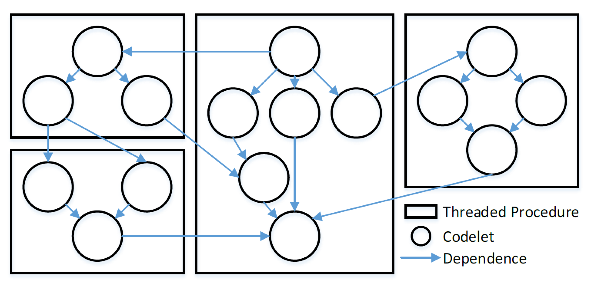
\includegraphics[]{Fig/figure2.png}
\end{figure}
%\textcolor{red}{Figure 2}


\subsection*{Codelet Abstract Machine Model (AMM)} The Codelet Abstract Machine Model describes a hierarchical abstract computer structure that a Codelet model follows during execution, which is not a real computer architecture but rather a map of it. Codelet abstraction machine model consists of many computing nodes, each computing node contains a number of multi-core chips, each multi-core chip is divided into a several clusters. The Codelet AMM ensures that cores within the same cluster are physically near to each other and share same L3 cache. Each cluster includes two kinds of processing units: one scheduling unit (SU) and multiple computing units (CUs). Data transmission under the node level leverages the shared address memory space. Each cluster contains a pending execution Codelet queue that stores the Codelet ready to be executed. The role of the SU is to maintain the queue. Whenever a Codelet is fired, SU will add it to the queue and load the required data to the cluster's cache. When a CPU core is available, CU will take a Codelet from the queue and executes its instructions. Due to the pending execution Codelet queue, the processing units do not need to be all the same, which also ensures the scalability of Codelet model on heterogeneous systems. An overview of Codelet Abstract Machine Model is shown in Figure 3.

\begin{figure}[h]
\caption{Figure 3}
\centering
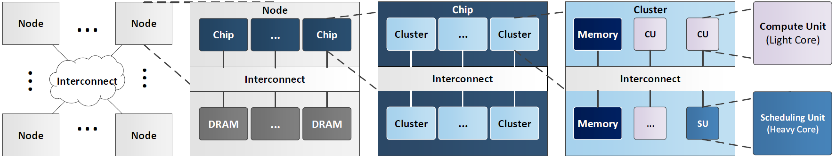
\includegraphics[width=1\textwidth]{Fig/figure3.png}
\end{figure}
%\textcolor{red}{Figure 3}

\subsection{Delaware Adaptive Run-Time System (DARTS)}
Since our main work is to apply Codelet model to brain-inspired computing, instead of implementing Codelet model, we borrowed DARTS - an implementation of Codelet model developed by the University of Delaware [4]. At present, a research team has already deployed it on Sunway supercomputer, the fastest supercomputer across the world, and conduct a serial of related research [5]. 
DARTS implements the Codelet AMM on real computer architectures for single-node shared memory multi-core computers from software level. With the help of DARTS, any existing computers can execute Codelet model under the node level. DARTS also allows users to set specific parameters of the abstract model, such as the number of clusters within a node, the number of CUs within a cluster, which allows us to conduct a more comprehensive analysis of the program performance. Moreover, DARTS has developed a complete runtime for Codelet model, including the implementation of Codelet and TP, the signal transmission among Codelets, and the different scheduling strategies of Codelet and TP.
DARTS is written in C ++ and uses a modular design that is highly portable and scalable. This is convenient not only to directly use the module, but also to improve the related modules for the brain-inspired computing features. (DARTS is an open source project, source code can be found here  \href{http://www.capsl.udel.edu/codelets/downloads/darts_20150318.tar.gz}{DARTS Source Code})


\section{Methodology}
\label{sec:method}
In this section, we introduce the Codelet model based brain-inspired computing platform taking artificial neural network for example. Due to the directed connected structure of artificial neural network is very similar to that of Codelet graph, we map the components of artificial neural network to corresponding components of Codelet model.
\subsection{Neuron}
Neuron is the basic element of artificial neural network. Its operating mechanism is shown in Figure 4. It takes the outputs of the predecessor neuron as inputs, add them to the weighted sum, activate it through non-linear functions and sent the output to the subsequent neuron, which is similar to the firing mechanism of Codelet. So we model neurons as Codelets, allowing Codelet to perform different neural functions by inheriting from the Codelet class and overloading the fire() function. 
 
%\textcolor{red}{Figure 4}
\begin{figure}[h]
\caption{Figure 4}
\centering
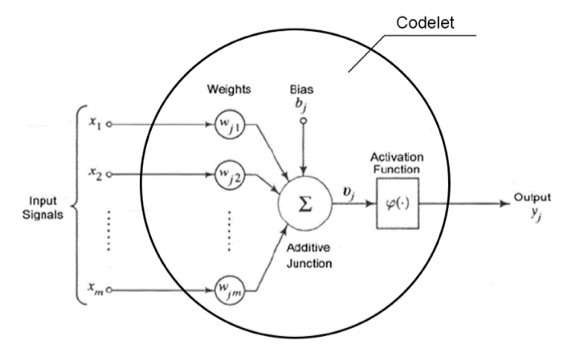
\includegraphics[width=1\textwidth]{Fig/figure4.png}
\end{figure}

Considering the overhead of Codelets executing on CUs, modeling each neuron as a Codelet will waste a lot of CPU time to switch between Codelets and reduce efficiency. On the other hand, modeling too many neurons as a Codelet loses the advantage of fine-grained parallel scheduling. After experimenting, we found that modeling 10-15 neurons as a Codelet can make the parallel computing achieve the highest efficiency.

\subsection{Layer}
Neurons in the artificial neural network are clustered into layers and neurons in the same layer perform the similar function and rely on the same input data. For some special types of neural layers, such as convolution layers, the neurons share the weights. Intuitively, the memory access time can be reduced by pre-loading shared input data or shared parameters between neurons into the cache, which is similar to the role of TP in the Codelet model. Therefore, we model the neural layer as a TP, which is inherited from the ThreadedProcedure class, and assign the corresponding local data storage area and the corresponding function's Codelet according to the type of the neural layer. Currently supported neural layer types are: convolutional layer, fully connected layer, pooling layer, Softmax classifier. An overview of layer built as TP is shown in Figure 5. The local data stores input data required by neurons, the weight parameters and the output data. Neurons only communicate with the local data, while the local data is responsible for data transmission between layers.
 
%\textcolor{red}{Figure 5}
\begin{figure}[h]
\caption{Figure 5}
\centering
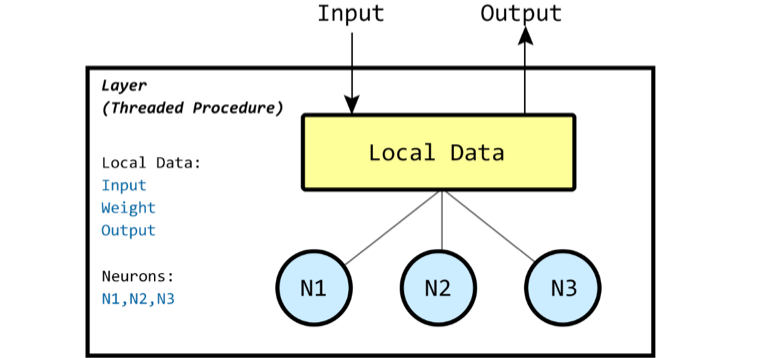
\includegraphics[width=1\textwidth]{Fig/figure5.png}
\end{figure}

\subsection{Signal/Data Transmission}
Because DARTS is based on shared address memory space, data transmission is completed by shared memory, while the signal transmission is complete by function call.
 
%\textcolor{red}{Figure 6}
\begin{figure}[h]
\caption{Figure 6}
\centering
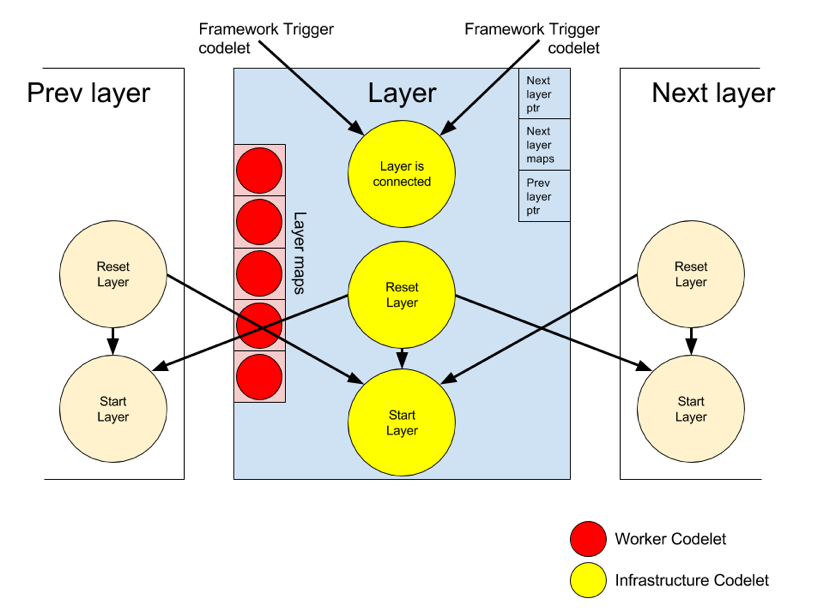
\includegraphics[width=1\textwidth]{Fig/figure6.png}
\end{figure}
Figure 6 shows the connection between a neural layer with its precursor and subsequent layer. Each layer contains the Codelets and local data. The red cells represent the working Codelet, responsible for the computation. The yellow cells represent the synchronous Codelet, responsible for the construction of the data signal transmission path between the Codelets. The local data contains relevant data, as well as the Codelet address that belong to precursor and subsequent layer which will be used for the construction of the data signal transmission path. When a layer is initialized, it will first confirm its connection with the precursor and subsequent layer via Codelet LayerIsConnected, and obtain the Codelet addresses of precursor and subsequent layer. Codelet ResetLayer and StartLayer play a role of synchronization in the pipeline execution. To avoid data racing during the pipeline execution, the layer ready to be executed and its subsequent layer should be reset. Therefore, when all the Codelets of a layer finish calculating, Codelet ResetLayer will be reset the Layer and signal Codelet StartLayer of itself, its precursor and its subsequent layer. When Codelet StartLayer collects three signals, it sets Codelets of the three layers as executable and waits to be fired by precursor Codelets.

\subsection{Construction and Execution of Neural Network}
As have introduced in Section 3.2, TP can be regarded as an asynchronous function call that provides a way to construct a CDG. Thus, we use a class Framework that calls TPs of all the layers in a network to construct a Codelet Graph that corresponding to the network. When a complete neural network framework is set up, the data flows in the framework in a pipelining manner.
In order to give full play to the advantages of asynchronous execution model, a Codelet will directly send signals to the subsequent Codelet after the completion of itself without waiting for the completion of the entire layer. Likewise, Codelet does not have to wait for the entire Codelet to start. Once all the input dependencies are satisfied, the Codelet will directly be added to the pending executed Codelet queue. In general, all Codelets are executed asynchronously and there is no specific synchronization point. 

\subsection{Multi-Framework Concurrency}
Although we have subdivided the parallel processing granularity into neuron levels, due to the structure of the neural network, the number of concurrent codelets to be executed may be less than the currently available number of computing units, i.e. the computing power is not fully utilized. For example, for the neural network shown in Figure 7, the maximum number of codelets to be executed at the same time is only 5 (the hidden layer neurons are all activated). If the computer has more than 5 computing units, the excess computing units remain idle. Therefore, we adopted a second-level parallel architecture, calling multiple frameworks simultaneously, i.e. processing multiple samples concurrently to make full use of all computing units. Since multiple frames use the same set of neural network parameters, the set of parameters should be stored in the main program and passed from the main program to each frame, as shown in Figure 8.
 
%\textcolor{red}{Figure 7}
\begin{figure}[h]
\caption{Figure 7}
\centering
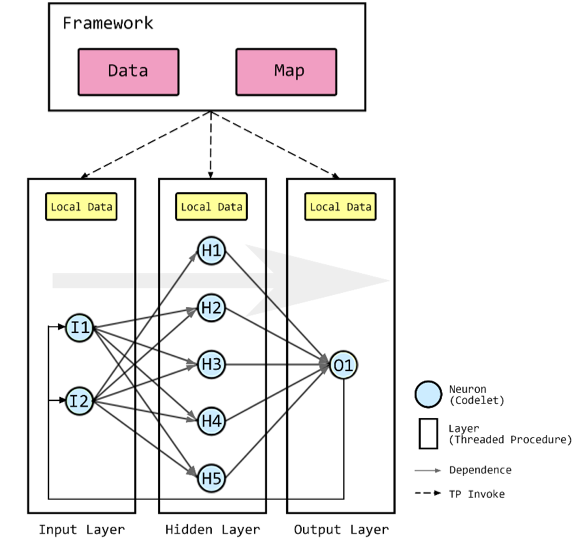
\includegraphics[width=1\textwidth]{Fig/figure7.png}
\end{figure}
 
%\textcolor{red}{Figure 8}
\begin{figure}[h]
\caption{Figure 8}
\centering
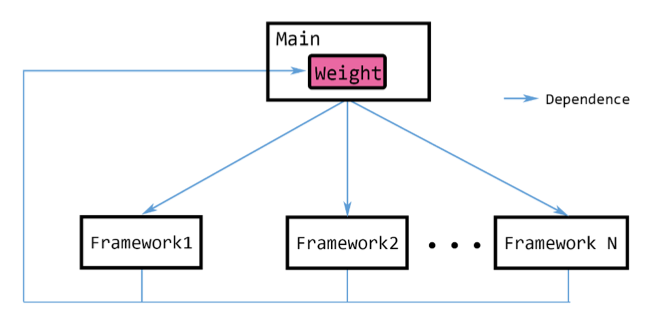
\includegraphics[width=1\textwidth]{Fig/figure8.png}
\end{figure}

\subsection{Training and Inference}
For the training of neural networks, we use batch training. Each batch of samples is distributed to all the frameworks and executed in parallel. When all the samples from a batch finish executing, the main program updates the parameters and then starts the next batch of sample training. The data flow diagram is shown in FIG. 6. For the inference of neural network, the output of each sample can be directly output without any data exchange because the inference of each sample is independent to each other.


\section{System Setup}
\label{sec:system}
Since DARTS only supports single-node computing systems, we integrate DARTS with Tensorflow to extend our platform to distributed computing systems. Figure 9 shows a schematic diagram of the DARTS-Tensorflow system. We embed the DARTS runtime system into Tensorflow's runtime system. For distributed systems, Tensorflow allocates computation tasks to each Node, and then DARTS is responsible for the internal computing work of each node.

%\textcolor{red}{Figure}
\begin{figure}[h]
\caption{Figure 9}
\centering
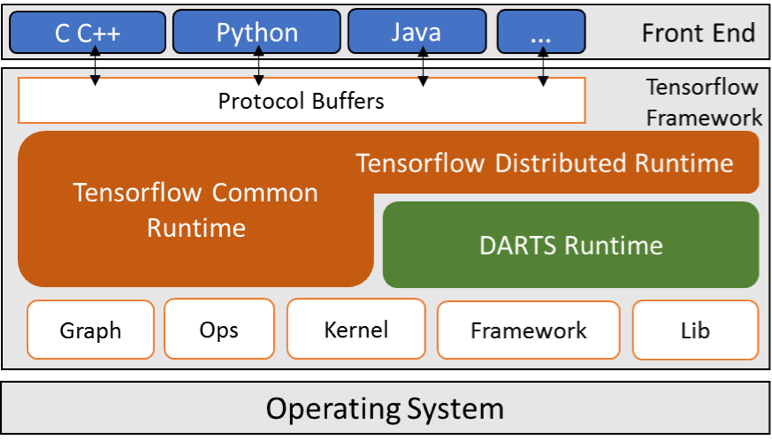
\includegraphics[width=1\textwidth]{Fig/figure9.png}
\end{figure}

\section{Experiments and Results}
\label{sec:results}
In this section, we will demonstrate our brain-inspired simulation platform in terms of efficiency and scalability. Efficiency refers to how much speed up our platform can bring, compared to serial execution. Scalability refers to whether execution efficiency can increase as the number of available computing unit increases. 
As an example, we use the Lenet-5, a 7-layer convolutional neural network for handwritten digit recognition to test the performance of our brain-inspired simulation platform. Lenet-5 was proposed by Yann LeCun et al [6] and considered as the most classic convolutional neural network, which can achieve more than 98\% recognition accuracy on the MINST dataset. Its importance of brain-inspired calculation is self-evident. We believe that if we can implement Lenet-5 in our platform and achieve high speed than the existing technology, it will be sufficient to prove the feasibility and superiority of brain-inspired computation simulation based on data flow.
In contrast, we choose OpenMP, a pervasively used coarse-grained multi-threaded parallel computing model, to implement Lenet-5. The parameters of OpenMP have been carefully tuned to achieve the best performance

\subsection{Testbed}
The CPU of our testbed is dual sockets Intel(R) Xeon(R) CPU E5-2670 @ 2.60GH. Each sockets consists of 8 cores (16 threads). Each core has 32KB L1 cache and 256KB L2 cache. Each socket shares 20MB L3 cache. Testbed uses CentOS Linux system. All the source code is compiled on GCC4.6.2.
\subsection{Results}
 
%\textcolor{red}{Figure 10}
\begin{figure}[h]
\caption{Figure 10}
\centering
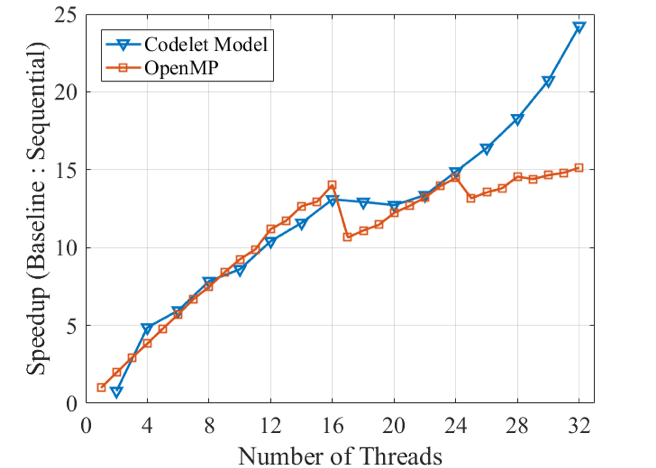
\includegraphics[width=1\textwidth]{Fig/figure10.png}
\end{figure}
Figure 10 shows the performance of two different implementation of Lenet-5 (Codelet model, OpenMP model). We manually change the number of thread and record the speed up against the sequential execution baseline. 
We can observe that when the number of threads available is less than 16, the speed up of both methods are comparable. However, when the number of threads increase over 16, the speed up of OpenMP shows a significant decrease. The reason lies in the dual-socket CPU employed by the testbed. Each socket has 16 threads, and no cache is shared between the sockets. When the computation work is allocated across the two sockets, all related data need to be read from the memory twice and synchronization operations will flush the cache twice, which will slow down the program. Our platform, on the other hand, is little effected by this situation. There are two main reasons: First, each TP stores the local data that are required by Codelets. These data need only be read into the cache once, saving memory access time; Second, the Codelet Abstract Machine Model ensures that the codelets within a TP can only run in the same cluster. Since the cluster is divided according to the processor hardware structure, which guarantees that Codelets from the same TP share the same L3 cache, there will be far less cache miss during execution.
When the number of available threads reaches more than 24, the execution efficiency of Codelet model begins to exceed that of OpenMP. When the number of threads reaches 32, the Codelet model provides 60% higher speed up than OpenMP, which shows that our platform has better scalability than OpenMP on multi-core and even many-core computing system.
We also examine the performance of our system against Tensrflow. The result is shown in Figure 11. The maximum speed up achieves 52.9%. We can conclude that, similar to the result against OpenMP, our platform demonstrates higher efficiency and scalability than Tensorflow. 
 
\textcolor{red}{Figure 11}
\begin{figure}[h]
\caption{Figure 11}
\centering
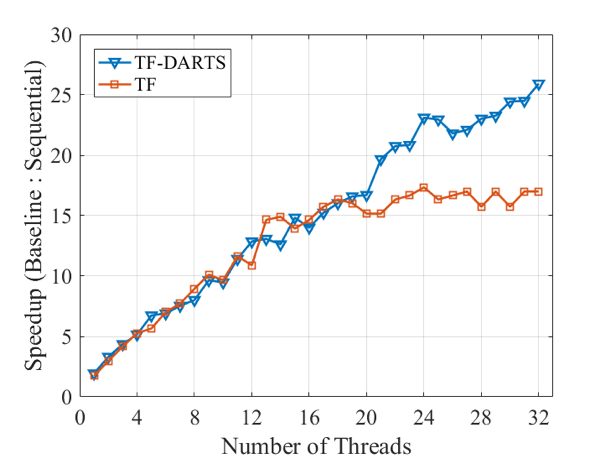
\includegraphics[width=1\textwidth]{Fig/figure11.png}
\end{figure}
In general, our platform, either alone or in combination with Tensorflow, shows higher efficiency and better scalability. Due to the fact that development of processor in the future is bound to increase core number, Codelet-based parallel brain-inspired computing simulation platform will have broader application prospects than traditional parallel acceleration model such as OpenMP.


\section{Conclusions}
\label{sec:conclusions}
Based on Codelet model, we proposed a novel brain-inspired computing simulation platform through the fine-grained multi-thread scheduling policy and asynchronous execution strategy, our platform provide a new path to solve the bottleneck facing the traditional parallel computing technology when they are applied to multi-core system.
We select LeNet-5, the most classic convolution neural network, as an example to demonstrate the high efficiency and scalability of our platform. Compared to sequential execution, the maximum speed up reaches 23.8 times. Compared to OpenMP, the maximum speedup reaches 1.6 times. By combining DARTS with Tensorflow, we extend our platform to distributed computing system. Results shows that the fusion system performs better than single Tensorflow by 52.9%.
To further justify the superiority and scalability of our framework, we would like to test our framework on the larger neural networks, such as GoogleNet and ResNet. We may also deploy our framework on a real dataflow processor such as Intel CSA instead of simulating on the current von Neumann architecture and x86 CPU. In this way, we expect the dataflow program execution model can be better fit into the underlying hardware without introducing additional overhead, leading to better parallel acceleration.


{\footnotesize \large
\bibliographystyle{abbrvnat}
\bibliography{bib/capsl,bib/others,bib/fsharp,bib/referencesUCI,bib/my_ref,bib/referencesUD}}

\end{document}
